%% Proposal
% Author: Hannah O'Sullivan h.osullivan18@imperial.ac.uk
% Date: Dec 18
% Script: Proposal.tex
% Desc: A laTex document outlining my project proposal

\documentclass[
11pt, % Define font
onehalfspacing, % Use onehalfspacing
parskip, % to add space between paragraphs
headsepline, % Get a line under the header
]{article} % The class file specifying the document structure
%\usepackage[backend=bibtex,style=authoryear,natbib=true]{biblatex} % Use the bibtex backend with the authoryear citation style (which resembles APA)
%\addbibresource{example.bib} % The filename of the bibliography
\usepackage[english]{babel}
\usepackage[T1]{fontenc} % to use the £ sign
\usepackage[math]{iwona} % to use the £ sign
\usepackage{helvet}
\renewcommand{\familydefault}{\sfdefault} % to get arial font
\usepackage{geometry}
\newcommand{\HRule}{\rule{\linewidth}{0.5mm}} % to get lines
\usepackage[hidelinks]{hyperref} % hide ugly blue box around links
\usepackage{microtype} %helps with end line word breaks
\usepackage[utf8]{inputenc} % file encoding
\usepackage{graphicx} % embed PDF
\usepackage{float} % to position figures
\usepackage{natbib} % flexible citations
\bibliographystyle{plainnat} % plain bibliography
\usepackage{lineno} % add line numbers
\usepackage{enumerate}

%% Add geometry
\geometry{
	paper=a4paper,
	inner=2cm, % Inner margin
	outer=2cm, % Outer margin
	bindingoffset=.5cm, % Binding offset
	top=2cm, % Top margin
	bottom=2cm, % Bottom margin
}

\begin{document} % Begin document
\date{} % Gets rid of the date randomly appearing
\begin{titlepage} % Set up title page
\begin{center} % Centre text

\vspace*{.06\textheight}
{\scshape\LARGE Imperial College London\par}\vspace{1.5cm} % University name
\textsc{\Large Master of Research Project Proposal}\\[0.5cm] % Document type

\HRule \\[0.4cm] % Horizontal line
{\huge \bfseries A new tool for quantifying the response of metabolic traits to climate change\par}\vspace{0.4cm} % Thesis title
\HRule \\[1.5cm] % Horizontal line

\begin{minipage}[t]{0.4\textwidth}
\begin{flushleft} \large
\emph{Author:} \\
%\author{Hannah O'Sullivan}
\supervisor{Hannah O'Sullivan} % will not accept author!!!
\href{mailto:h.osullivan@imperial.ac.uk}{h.osullivan@imperial.ac.uk}
\end{flushleft}
\end{minipage}
\begin{minipage}[t]{0.4\textwidth}
\begin{flushright} \large
\emph{Supervisor:} \\
\supervisor{Dr. Samraat Pawar}
\href{mailto:s.pawar@imperial.ac.uk}{s.pawar@imperial.ac.uk}
\end{flushright}
\end{minipage}\\[3cm]

\vfill

{\large \today}\\[4cm] % Date

\vfill
\end{center}
\end{titlepage}

\begin{linenumbers}
\maketitle
\section*{Keywords}
\emph{Ecoinformatics; Metabolic theory; Climate change; Mathematical modelling; Temperature; Ecology.}


\maketitle
\section*{Introduction}
Temperature is fundamental to the rate at which energy and materials are reorganised in individuals, communities and ecosystems \citep{Brown2004}. The intrinsic function of temperature in ecology allows for insights into how biological systems might respond in the face of an ever changing thermal environment. In recent years, a wealth of research has been produced using intraspecific and interspecific thermal responce curves to understand biological responses to temperature \citep{Dell2011} \citep{Thomas2012}. However, far less research has been devoted to assessing the quantitative tools available to researchers striving to answer this complex question. Given the importance of thermal response curves in the context of global climate change, it is imperative to approach data analysis with precision and care. For example, biogeographical estimates derived from the same data, with even the best-fitting models, have differed by the equivalent of a decade of predicted warming \citep{Low-Decarie2017}. Significant fluctuation in results can also arise due to the quality of data used in fitting models. One key example of this, is the difference found in activation energy estimates due to variation in the range or frequency of temperatures measured \citep{Pawar2016}.
Thus, this project aims to reevaluate the models available to metabolic theorists and assess them given the data accessible today. In addition to this, I aim to construct an innovative tool to aid in the model fitting of thermal performance curves and encourage overlap of practice between researchers in this field.

\maketitle
\section*{Methods}
The data used in this project will be taken from the published BioTraits database \citep{Dell2013}. Firstly, the scope of data quality will be investigated with two parameters; the range of temperature values taken and the frequency with which these values are recorded. Following this, the current mathematical models pertaining to metabolic theory will be implemented into Python modules. At this stage, it will be possible to compare the performance and precision of each model to various levels of data quality using maximum likelihood and bayesian methods. In understanding the shortcomings of both data and models at this basal level, it will then be possible to make assessments of model robustness at higher level of realism. Rigorous testing of the Python modules will ensure transparency and cross-platform compatibility. Eventually, these will be synthesised into a concise package as away of distributing a relevant collection of mathematical models for general use.

\maketitle
\section*{Anticipated outcomes and results}
This project aims to assess the flaws and shortcomings in the current quantitative tools used for analysing thermal responses. It will investigate the importance of precision, over generality and reality in the model fitting process. In the creation of a python package, I aim to inform decision making and efficiently contribute a robust set of computational methods to peers. In addition to this, the software tool will allow for elucidating higher level ecological questions such as population and coevolutionary dynamics.

\maketitle
\section*{Project feasibility}
\begin{figure}[H]
      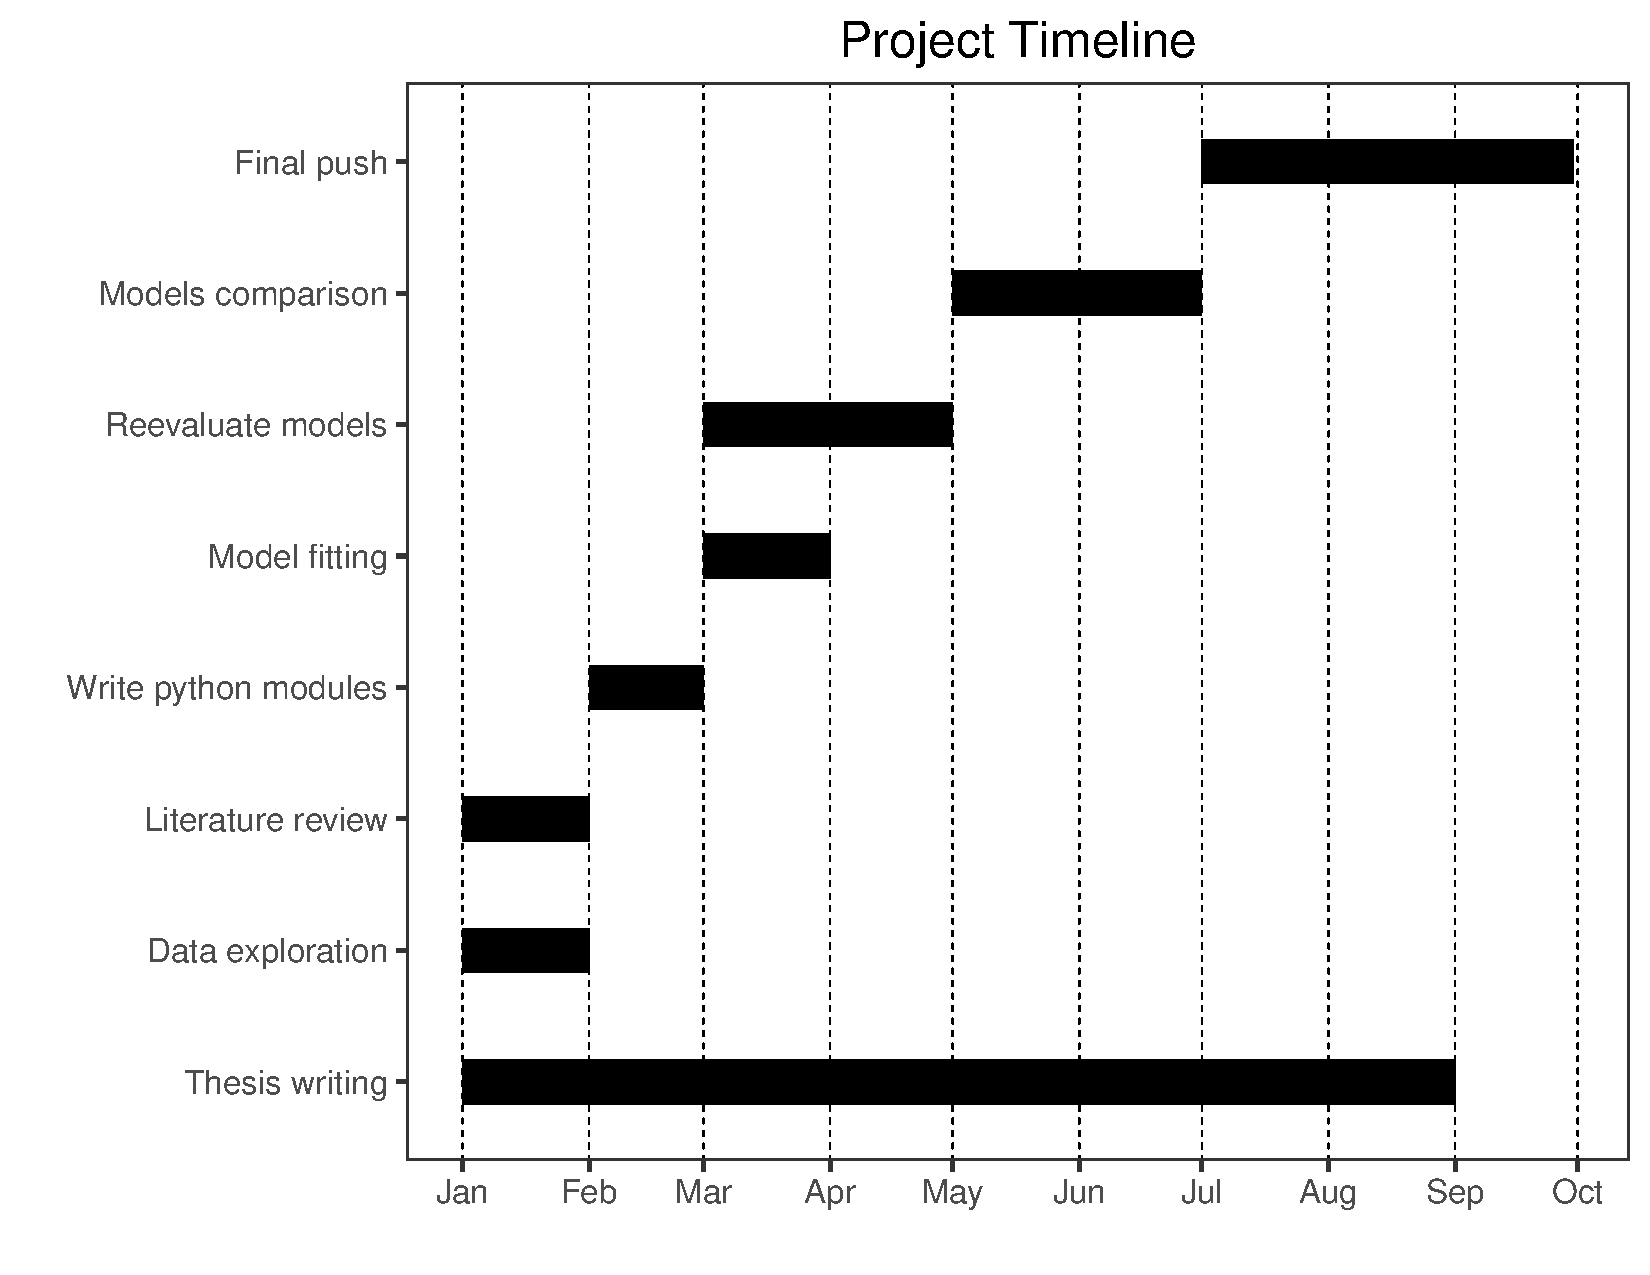
\includegraphics[width = 1\textwidth]{../Data/gantt_new.PDF}
      \caption{A Gantt chart outlining the approximate amount of time given to each main task between Januray 2019 and September 2019.}
\end{figure}


\maketitle
\section*{Budget}
\begin{enumerate}
	\item Train fare(£150):
	\begin{enumerate}
		\item Covers approximately three trips to Falmouth, Cornwall.
		\item Necessary for ongoing collaboration with researchers at the Penryn Campus, Universty of Exeter.
	\end{enumerate}
	\item External hard drive (£50):
	\begin{enumerate}
		\item To back up large volumes of data throughout the course of the project.
\end{enumerate}

\end{linenumbers}

\pagebreak % new page for bibliography

\bibliography{../Data/Proposal.bib}

\pagebreak % New page for supervisor signature

%\begin{minipage}[t]{0.4\textwidth}
\begin{flushright} \large
\mbox{} % something above vfill to make it work
\vfill
\emph{I have seen and approved the proposal and budget:} \\
\vspace{10mm} % spacing for signature and date
\noindent\begin{tabular}{ll}
\makebox[2.5in]{\hrulefill} & \makebox[2.5in]{\hrulefill}\\
Supervisor & Date\\
\end{tabular}
\end{flushright}
%\end{minipage}\\[3cm]



\end{document}
